\documentclass{article}
\usepackage{tikz}
\usetikzlibrary{shapes.geometric, arrows, positioning, calc}

\begin{document}

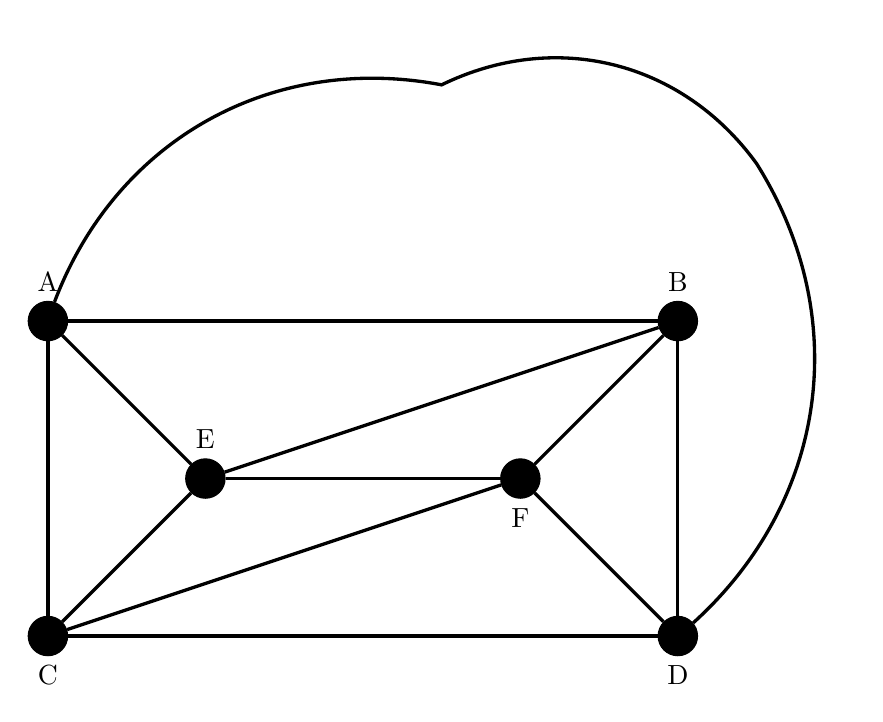
\begin{tikzpicture}
\node[draw,circle,fill=black,label=above:E,minimum size=0.5cm] (e) at (0,0){};
\node[draw,circle,fill=black,label=below:F,minimum size=0.5cm] (f) at (4,0){};
\node[draw,circle,fill=black,label=above:B,minimum size=0.5cm] (b) at (6,2){};
\node[draw,circle,fill=black,label=above:A,minimum size=0.5cm] (a) at (-2,2){};
\node[draw,circle,fill=black,label=below:D,minimum size=0.5cm] (d) at (6,-2){};
\node[draw,circle,fill=black,label=below:C,minimum size=0.5cm] (c) at (-2,-2){};

\draw[very thick] (a) to (e);
\draw[very thick] (e) to (f);
\draw[very thick] (f) to (d);
\draw[very thick] (c) to (e);
\draw[very thick] (f) to (b);

\draw[very thick] (a) to (c);
\draw[very thick] (c) to (d);
\draw[very thick] (d) to (b);
\draw[very thick] (a) to (b);

\draw[very thick] (e) to (b);
\draw[very thick] (c) to (f);

\draw[very thick,bend left=40] (a) to (3,5) to (7,4) to (d);
\end{tikzpicture}
\end{document}